\chapter{Multiple Input Multiple Output Multi-path}

we will do as we did in SISO here.
\begin{enumerate}
	\item graphical representation of the system
	\item bulding the scattering maxrex for each frame and calculating the BER for each Eb/No
	\item plotting the relationship between BER and Eb/No for the MIMO system.
\end{enumerate}

\section{Graphical implementation}
before simulating the system we need first to be more familiar with multi-path system we will plot the multi path system we created Figure[\ref{fig:MIMO-multipath}].


\begin{figure}[!h]
	\centering
	
\includegraphics[width=0.7\linewidth]{"figures/MIMO Multipath.pdf"}
	\caption{}
	\label{fig:MIMO-multipath}
\end{figure}


\subsection{Simulating the system}
in this stage, we are re-simulating the system for each frame and calculating the average BER for each Eb/No.

\section{Plotting}
after simulating the system and getting all the values needed, we are ploting the relationship between the BER and Bb/No for SISO, SIMO, MIMO multi-path systems to see the diffrence between them Figure[\ref{32345}].

and as we can see, the BER in MIMO is not only lesser than the BER in SIMO, but also has faster decline.

\begin{figure}[!h]
	\centering
	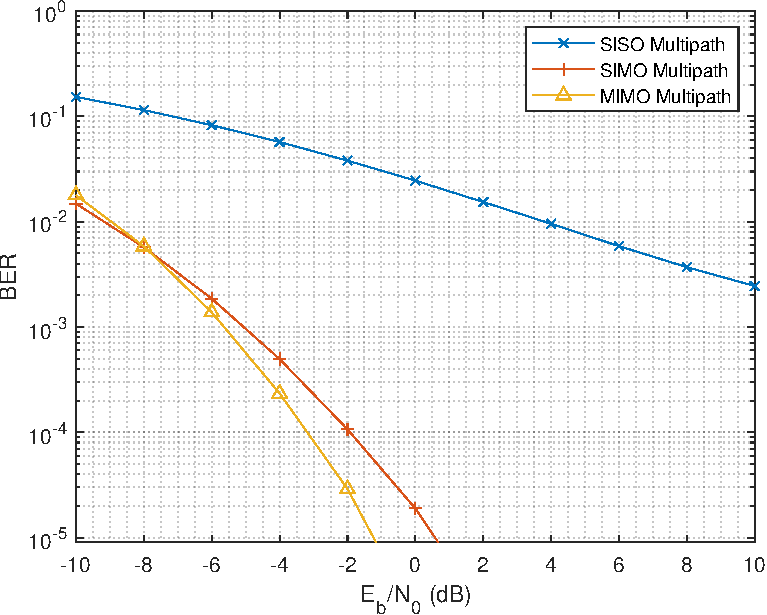
\includegraphics[width=1\linewidth]{figures/SISO_SIMO_MIMO Multipath.pdf}
	\caption{SISO LOC vs Multi-path}
	\label{32345}
\end{figure}



\newgeometry{margin=0pt}
\newpage
\vfill
\begin{figure}
	\centering
	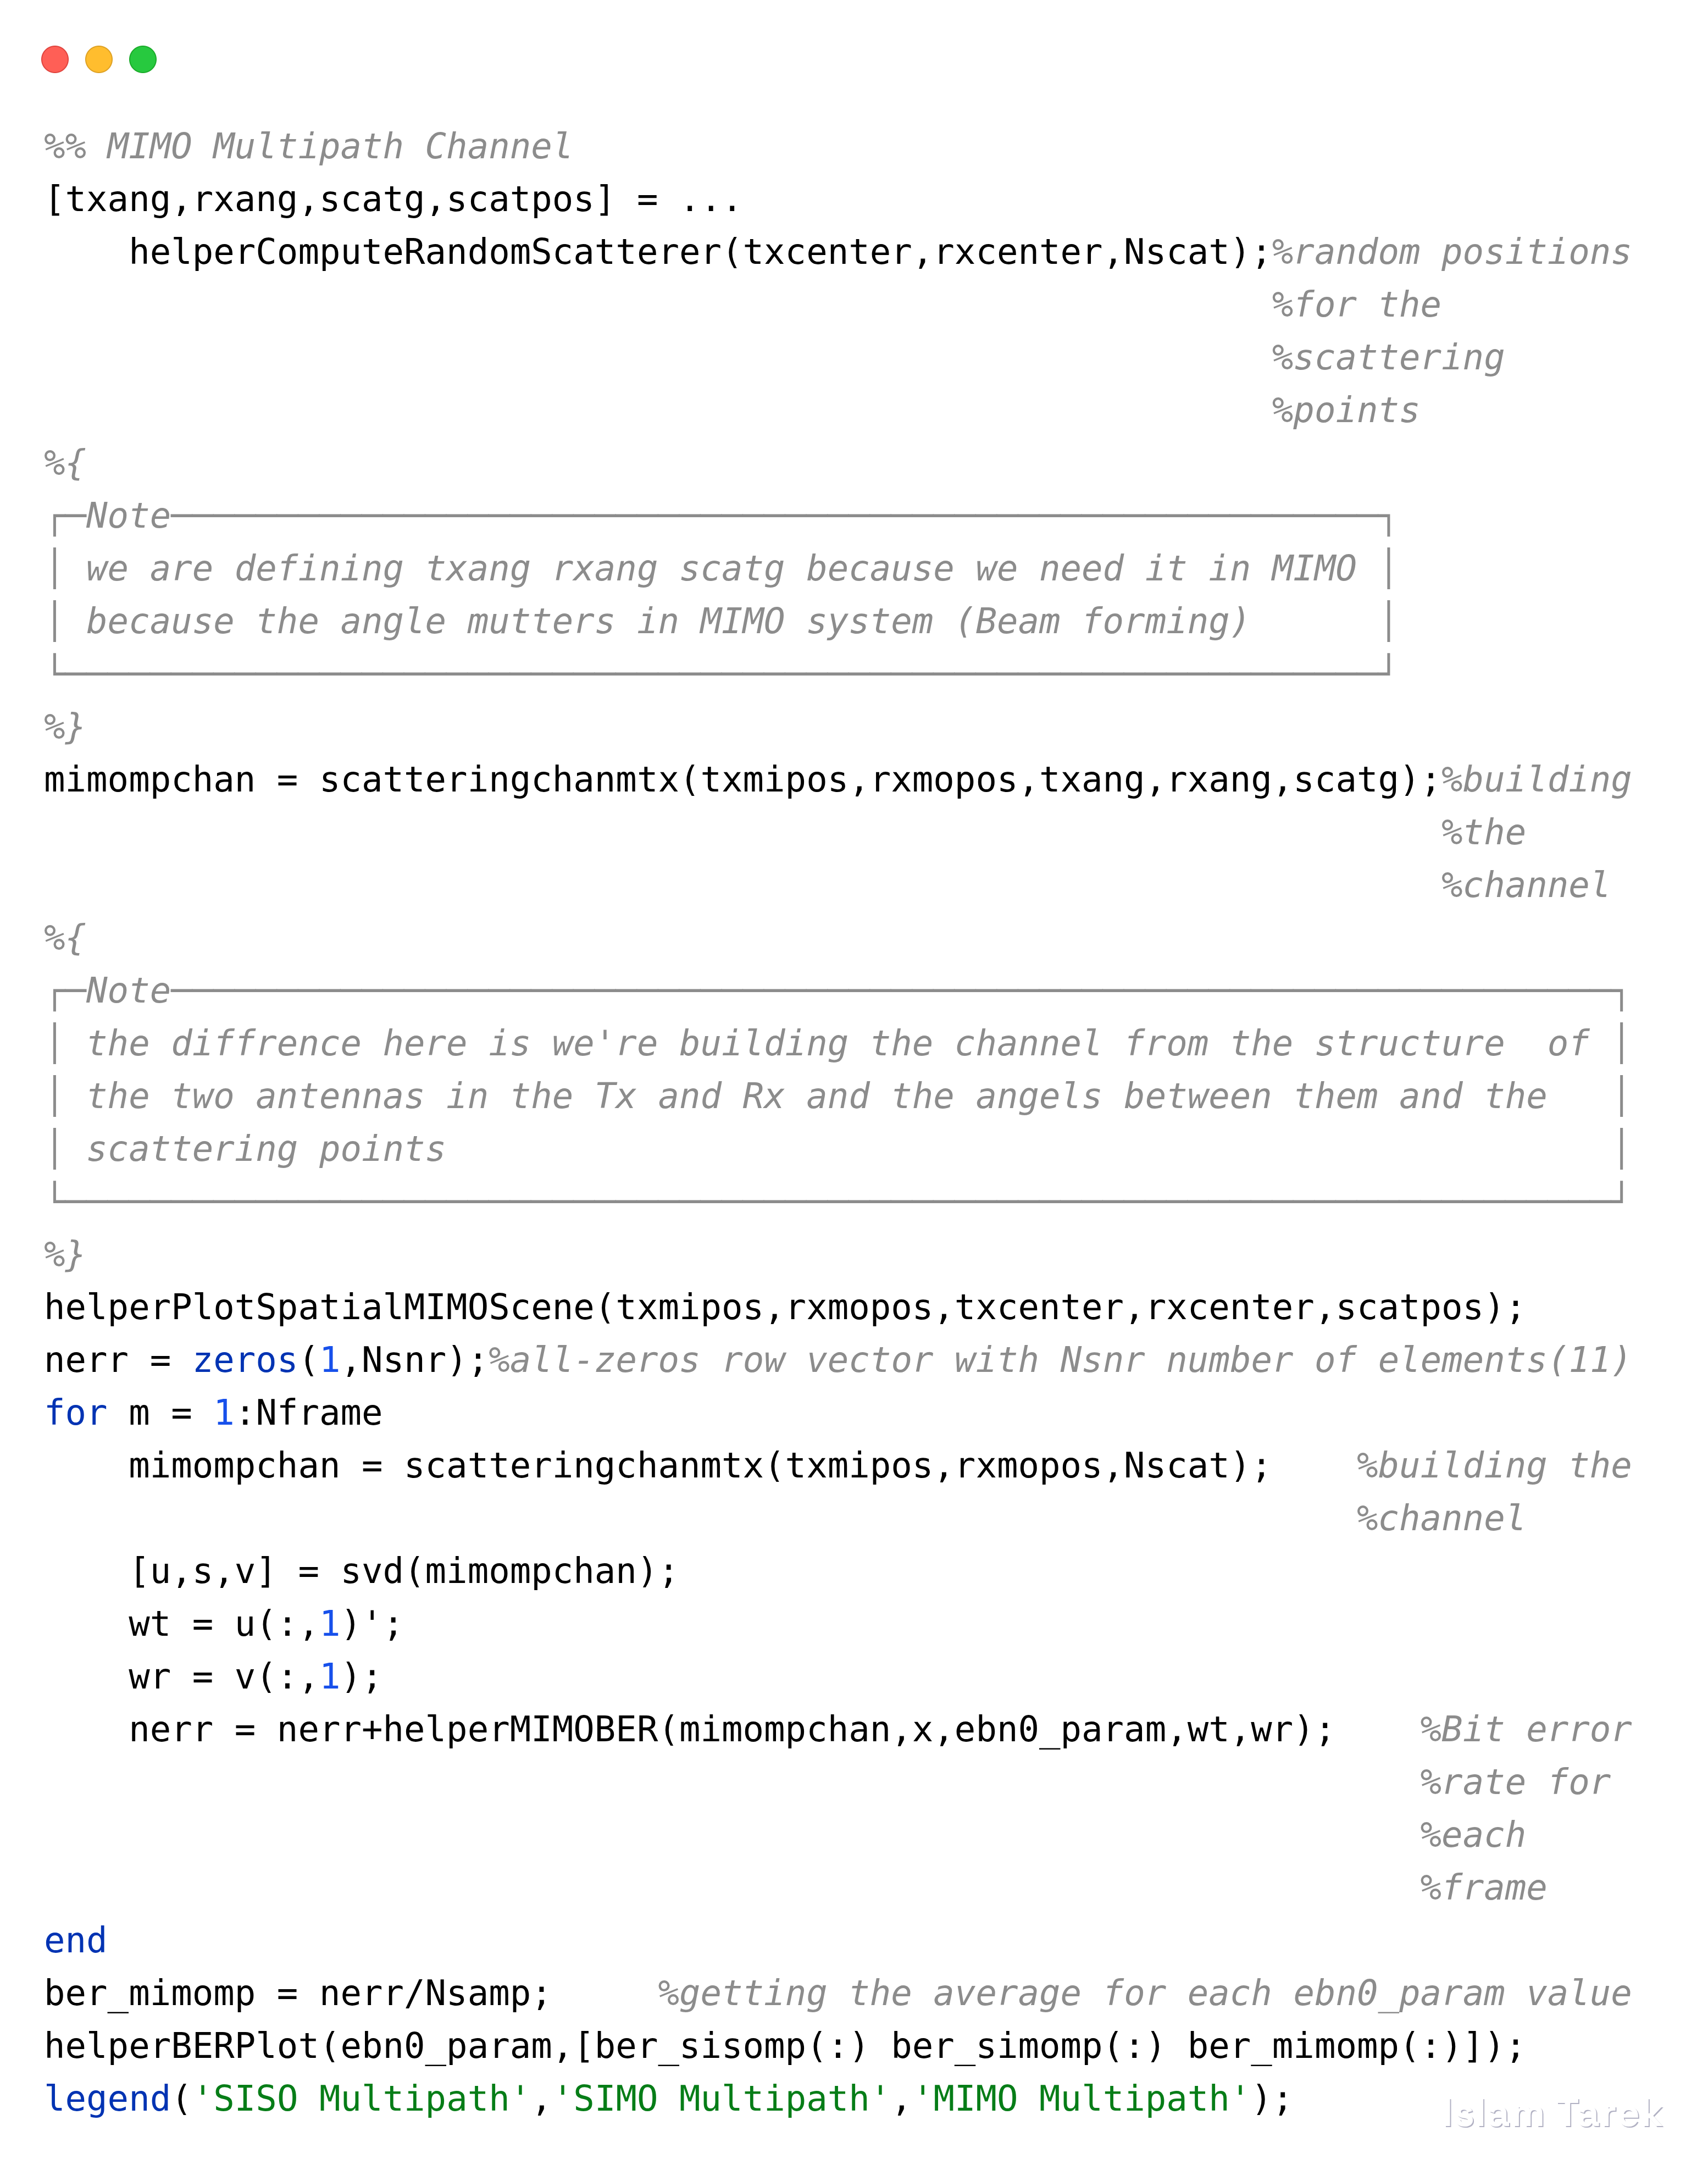
\includegraphics[width=0.7\linewidth]{figures/code9}
\end{figure}
\vfill
\restoregeometry